%
%
\documentclass[twoside,11pt]{../sty/report_petsc}

\usepackage{makeidx,xspace}
\usepackage[bookmarksopen,colorlinks]{hyperref}
\usepackage[all]{hypcap}
\usepackage{color}
\input pdfcolor.tex

\usepackage[pdftex]{graphicx}


\usepackage{times}
\usepackage{listings}
\usepackage{tikz}
%\usepackage{psfig}
\usepackage{../sty/verbatim}
\usepackage{../sty/tpage}
\usepackage{../sty/here}
\usepackage{../sty/anlhelper}
\usepackage[hyphens,spaces,obeyspaces]{../sty/trl}

\setlength{\textwidth}{6.5in}
\setlength{\oddsidemargin}{0.0in}
\setlength{\evensidemargin}{0.0in}
\setlength{\textheight}{9.2in}
\setlength{\topmargin}{-.8in}

\newcommand{\findex}[1]{\index{#1}}
\newcommand{\sindex}[1]{\index{#1}}
\newcommand{\A}{\mbox{\boldmath \(A\)}}
\newcommand{\F}{\mbox{\boldmath \(F\)}}
\newcommand{\J}{\mbox{\boldmath \(J\)}}
\newcommand{\x}{\mbox{\boldmath \(x\)}}
\newcommand{\bb}{\mbox{\boldmath \(b\)}}
\newcommand{\rr}{\mbox{\boldmath \(r\)}}
hyperbaseurl

\makeindex

% Defines the environment where design issues are discussed. In the manual
% version of this report, these regions are ignored.
\def\design{\medskip \noindent Design Issue:\begin{em}}
\def\enddesign{\end{em} \medskip}
% Manual version:
% \def\design{\comment}
% \def\enddesign{\endcomment}

% Print DRAFT in large letters across every page
%\special{!userdict begin /bop-hook{gsave 200 70 translate
%65 rotate /Times-Roman findfont 216 scalefont setfont
%0 0 moveto 0.95 setgray (DRAFT) show grestore}def end}

% Defines that we're doing the whole manual, not the short intro part,
% used in part1.tex.
\def\shortintro{false}

\usepackage{fancyhdr,lastpage}
\pagestyle{fancy}
\rhead{PETSc 3.6 \today}

\begin{document}


%%%%%%%%%%%%%%%%%%%%%%%%%%%%%%%%%%%%%%%%%%%%%%%%%%%%%%%%%%%%%%%%%%%%%%%%%%%%%%%%%%%%

\pagestyle{empty}
\hspace{-.65in}
\includegraphics{ArgonneLogo}
\hfill  {\large {\bf ANL-95/11 Rev 3.6}}

\vspace*{3in}
\noindent {\huge{\bf PETSc Users Manual}}
\vspace*{8pt}
\hrule
\vspace*{8pt}
\noindent {\Large{\it Revision 3.6}}

\vspace*{1in}
\noindent \\
{\Large {\bf Mathematics and Computer Science Division}}

\vspace*{10pt}


\vspace*{20pt}


%%%%%%%%%%%%%%%%%%%%%%%%%%%%%%%%%%%%%%%%%%%%%%%%%%%%%%%%%%%%%%%%%%%%%%%%%%%%%%%%%%%%

\newpage
\centerline{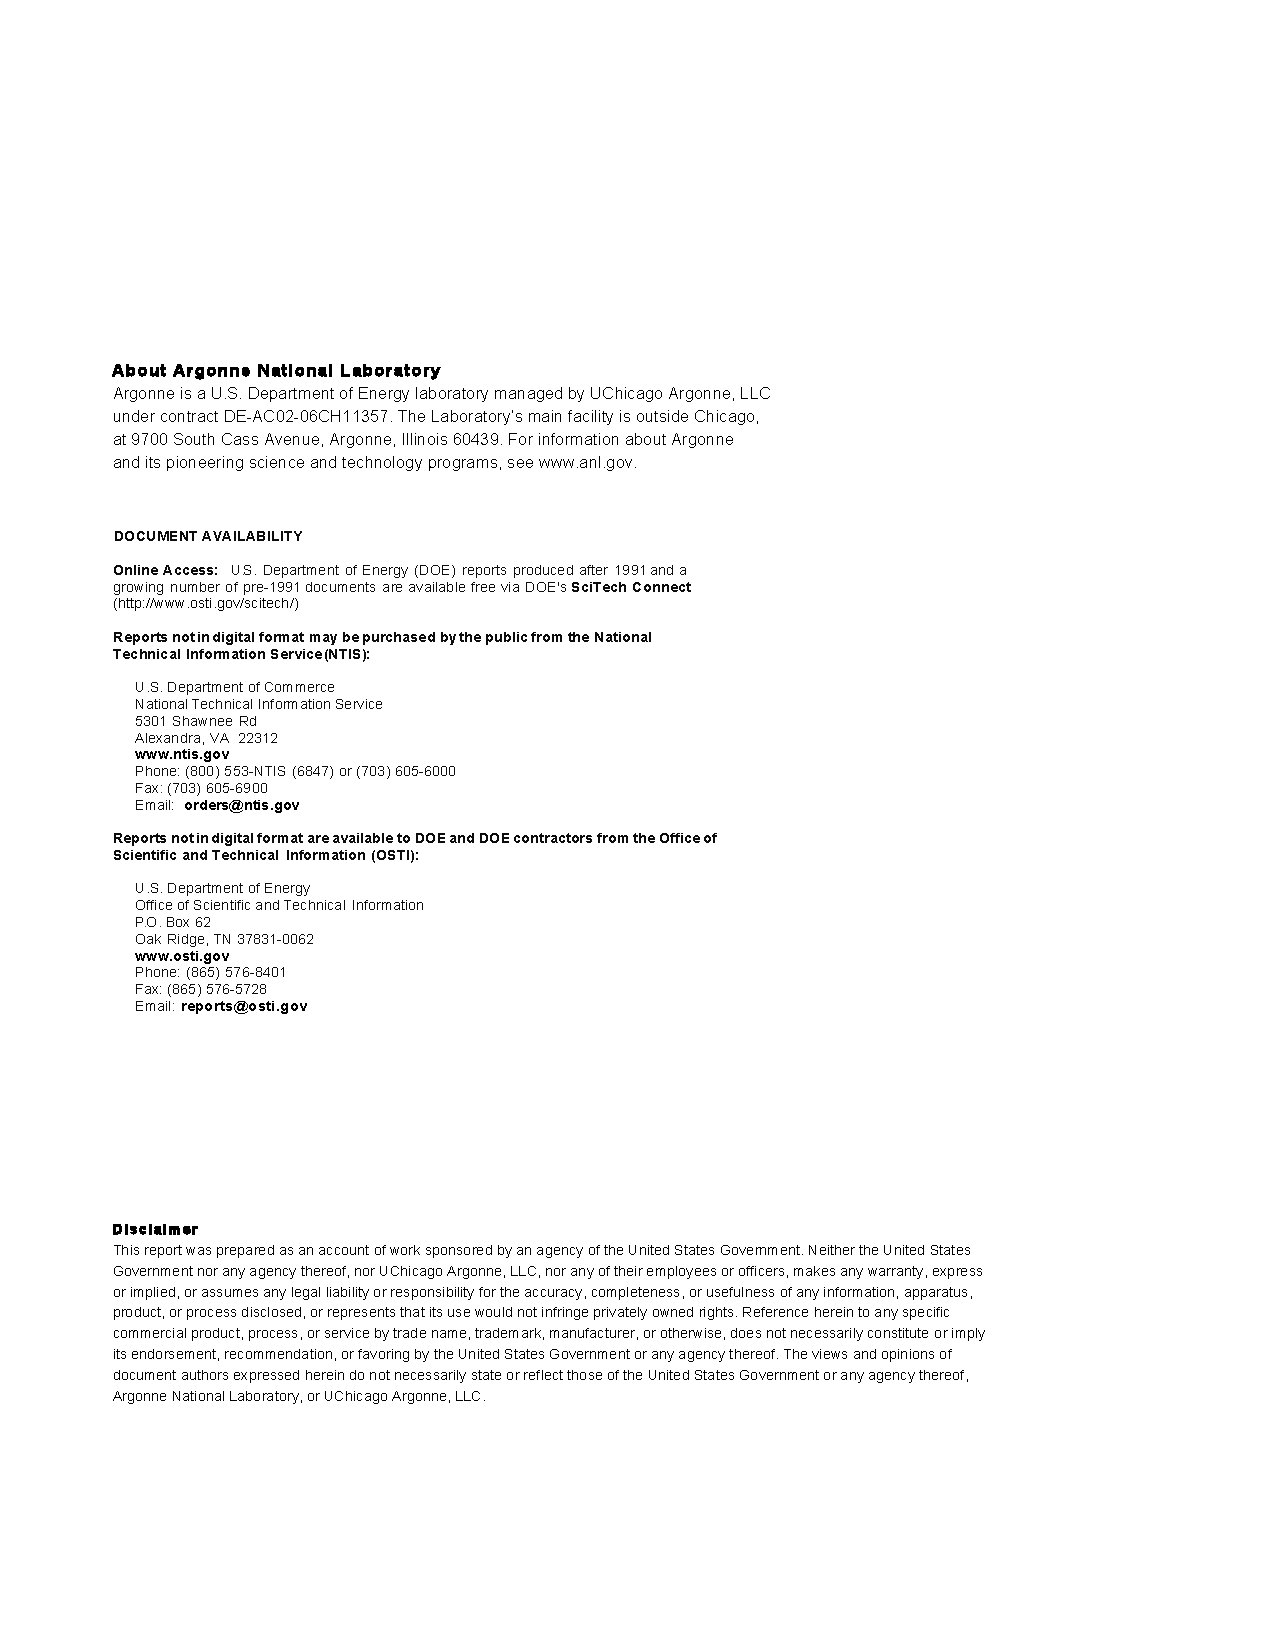
\includegraphics{ArgonneReportTemplatePage2}}
\newpage

\hfill {\large {\bf ANL-95/11 Rev 3.6}}

\vspace*{3in}
\noindent {\LARGE{\bf PETSc Users Manual}}
\vspace*{8pt}
\hrule
\vspace*{8pt}
\noindent {\Large{\it Revision 3.6}}

\vspace*{1in}
\noindent Prepared by \\
S. Balay, S. Abhyankar, M. Adams, J. Brown, P. Brune, K. Buschelman, L. Dalcin, V. Eijkhout, W. Gropp, D. Karpeyev,
D. Kaushik, M. Knepley, L. Curfman McInnes, K. Rupp, B. Smith, S. Zampini, and H. Zhang
Mathematics and Computer Science Division, Argonne National Laboratory

\vspace*{30pt}
\noindent June 2015

\vspace*{20pt}
\noindent This work was supported by the Office of Advanced Scientific Computing Research, \\
Office of Science, U.S. Department of Energy, under Contract DE-AC02-06CH11357.


\cleardoublepage
%\pagestyle{plain}
\pagestyle{fancy}
\vspace{1in}
\date{\today}

% Abstract for users manual
\addcontentsline{toc}{chapter}{Abstract}
% Abstract for PETSc Users Manual

%
%   Next line temp removed
%
\noindent {\bf Abstract:}

\medskip \medskip
This manual describes the use of PETSc for the numerical solution
of partial differential equations and related problems
on high-performance computers.  The
Portable, Extensible Toolkit for Scientific Computation (PETSc) is a
suite of data structures and routines that provide the building
blocks for the implementation of large-scale application codes on parallel
(and serial) computers.  PETSc uses the MPI standard for all
message-passing communication.

PETSc includes an expanding suite of parallel linear, nonlinear
equation solvers and time integrators that may be
used in application codes written in Fortran, C, C++, Python, and MATLAB (sequential).  PETSc
provides many of the mechanisms needed within parallel application
codes, such as parallel matrix and vector assembly routines. The library is
organized hierarchically, enabling users to employ the level of
abstraction that is most appropriate for a particular problem. By
using techniques of object-oriented programming, PETSc provides
enormous flexibility for users.

PETSc is a sophisticated set of software tools; as such, for some
users it initially has a much steeper learning curve than a simple
subroutine library. In particular, for individuals without some
computer science background, experience programming in C, C++ or Fortran and experience using a debugger such as \trl{gdb} or \trl{dbx}, it
may require a significant amount of time to take full advantage of the
features that enable efficient software use.  However, the power of
the PETSc design and the algorithms it incorporates may make the efficient
implementation of many application codes simpler than ``rolling
them'' yourself.
\begin{itemize}
\item  For many tasks a package such as MATLAB is often the best tool; PETSc is not
intended for the classes of problems for which effective MATLAB code
can be written. PETSc also has a MATLAB interface, so portions of your code can be written in MATLAB to ``try out'' the PETSc solvers.
The resulting code will not be scalable however because currently MATLAB is inherently not scalable.
\item PETSc should not be used to attempt to provide
a ``{\bf parallel linear solver}'' in an otherwise sequential code.
Certainly all parts of a previously sequential code need not be parallelized but the
matrix generation portion must be parallelized to expect any kind of reasonable performance.
Do not expect to generate your matrix sequentially and then ``use PETSc'' to solve
the linear system in parallel.
\end{itemize}

Since PETSc is under continued development, small changes in usage and
calling sequences of routines will occur.  PETSc is supported; see the
web site \href{http://www.mcs.anl.gov/petsc}{http://www.mcs.anl.gov/petsc} for information on
contacting support.

A \href{http://www.mcs.anl.gov/petsc/publications}{http://www.mcs.anl.gov/petsc/publications} may be found
a list of publications and web sites that feature work involving PETSc.


We welcome any reports of corrections for this document.

\medskip \medskip





\cleardoublepage


% ---------------------------------------------------------------------------
%

\medskip\medskip

\noindent {\bf Getting Information on PETSc:}

\medskip


\noindent {\bf On-line:}
\begin{list}{$\bullet$}
{
\setlength{\itemsep}{-.020in}
\setlength{\topsep}{0in}
\setlength{\partopsep}{0in}
}
\item Manual pages--example usage
\href{index.html}{docs/index.html}  or
\href{http://www.mcs.anl.gov/petsc/documentation}{http://www.mcs.anl.gov/petsc/documentation}
\item Installing PETSc
\href{http://www.mcs.anl.gov/petsc/documentation/installation.html}{http://www.mcs.anl.gov/petsc/documentation/installation.html}
\end{list}

\medskip
\noindent {\bf In this manual:}
\begin{list}{$\bullet$}
{
\setlength{\itemsep}{-.02in}
\setlength{\topsep}{.02in}
\setlength{\partopsep}{0in}
}
\item Basic introduction, page \pageref{sec_gettingstarted}
\item Assembling vectors, page \pageref{sec_vecbasic}; and matrices, \pageref{chapter_matrices}
\item Linear solvers, page \pageref{ch_ksp}
\item Nonlinear solvers, page \pageref{chapter_snes}
\item Timestepping (ODE) solvers, page \pageref{chapter_ts}
\item Index, page \pageref{ch_index}
\end{list}

% ---------------------------------------------------------------------------


\medskip \medskip

\cleardoublepage

% Acknowledgements for users manual
% Acknowledgements for TAO Users Manual
%
% These are also listed on the TAO homepage, so if you add something here
% add it to the home page also
%

\addcontentsline{toc}{chapter}{Acknowledgments}
\section*{Acknowledgments}

We especially thank Jorge Mor\'e for his leadership, vision, and effort on 
previous versions of TAO.  

TAO relies on PETSc for the linear algebra required to solve optimization
problems, and we have benefited from the PETSc team's experience, tools, 
software, 
and advice. In many ways, TAO is a natural outcome of the PETSc 
development.  

TAO has benefited from the work of various researchers who have provided 
solvers, test problems, and interfaces.  In particular, we acknowledge Lisa 
Grignon, Elizabeth Dolan, Boyana Norris, Gabriel Lopez-Calva, Yurii Zinchenko, 
Michael Gertz, Jarek Nieplocha, Limin Zhang, Manojkumar Krishnan, and Evan 
Gawlik.  We also thank all TAO users for their comments, bug reports, and 
encouragement.

The development of TAO is supported by the Office of Advanced Scientific 
Computing Research, Office of Science, U.S. Department of Energy, under 
Contract DE-AC02-06CH11357.  We also thank the Argonne Laboratory Computing 
Resource Center and the National Energy Research Scientific Computing Center 
for allowing us to test and run TAO applications on their machines.

%%% Local Variables: 
%%% mode: latex
%%% TeX-master: "manual_tex"
%%% End: 


% Blank page makes double sided printout look bettter.

\cleardoublepage

\tableofcontents

% --------------------------------------------------------------------
%                            PART 1
% --------------------------------------------------------------------
\cleardoublepage
\part{Introduction to PETSc}
\label{part_intro}
\cleardoublepage
\chapter{Getting Started}
\input{part1tmp.tex}

% --------------------------------------------------------------------
%                            PART 2
% --------------------------------------------------------------------
\cleardoublepage
\part{Programming with PETSc}
\label{part_usage}
\input{part2tmp.tex}


%------------------------------------------------------------------


\cleardoublepage
\bibliographystyle{plain}
\addtocounter{chapter}{1}
\addcontentsline{toc}{chapter}{Bibliography}
\label{sec:bib}
\bibliography{../petsc,../petscapp}

\pagestyle{empty}
\begin{figure*}[hbt]
\centerline{
\includegraphics{ArgonneReportTemplateLastPage.pdf}}
\caption{}
\end{figure*}

\end{document}
